\documentclass[12pt]{article}
\usepackage[english]{babel}
\usepackage{natbib}
\usepackage{url}
\usepackage[utf8x]{inputenc}
\usepackage{amsmath}
\usepackage{graphicx}
\graphicspath{{images/}}
\usepackage{parskip}
\usepackage{fancyhdr}
\usepackage{vmargin}
\setmarginsrb{3 cm}{2.5 cm}{3 cm}{2.5 cm}{1 cm}{1.5 cm}{1 cm}{1.5 cm}

\title{Design Driven Innovation}					% Title
\author{U.G.C.Jayasankha}								% Author
\date{\today}											% Date

\makeatletter
\let\thetitle\@title
\let\theauthor\@author
\let\thedate\@date
\makeatother

\pagestyle{fancy}
\fancyhf{}
\rhead{\theauthor}
\lhead{\thetitle}
%\chead{170259P}
\cfoot{\thepage}

\begin{document}

%%%%%%%%%%%%%%%%%%%%%%%%%%%%%%%%%%%%%%%%%%%%%%%%%%%%%%%%%%%%%%%%%%%%%%%%%%%%%%%%%%%%%%%%%

\begin{titlepage}
	\centering
    \vspace*{0.5 cm}
    
\includegraphics[scale = 0.8]{University_of_Moratuwa_logo.png}\\[1.0 cm]	% University Logo
    \textsc{Department of Electronics and Telecommunication Engineering University of Moratuwa}\\[0.8 cm]
    %\textsc{\Large University of Moratuwa}\\[1.0 cm]	% University Name
	\textsc{\Large En 3023}\\[0.3 cm]				% Course Code
	\textsc{\Large Electronic Design Realization}\\[0.5 cm]				% Course Name
	\rule{\linewidth}{0.2 mm} \\[0.4 cm]
	{ \huge \bfseries \thetitle}\\
	\rule{\linewidth}{0.2 mm} \\[1.5 cm]
	
	\begin{minipage}{0.4\textwidth}
		\begin{flushleft} \large
			\emph{Name:}\\
			\theauthor
			\end{flushleft}
			\end{minipage}~
			\begin{minipage}{0.4\textwidth}
			\begin{flushright} \large
			\emph{Index Number:} \\
			170259P									% Your Student Number
		\end{flushright}
	\end{minipage}\\[2 cm]
	
	{\large \thedate}\\[2 cm]
 
	\vfill
	
\end{titlepage}

%%%%%%%%%%%%%%%%%%%%%%%%%%%%%%%%%%%%%%%%%%%%%%%%%%%%%%%%%%%%%%%%%%%%%%%%%%%%%%%%%%%%%%%%%

\tableofcontents
\pagebreak

%%%%%%%%%%%%%%%%%%%%%%%%%%%%%%%%%%%%%%%%%%%%%%%%%%%%%%%%%%%%%%%%%%%%%%%%%%%%%%%%%%%%%%%%%

\section{Redefining a meaning of a product }
A normal standing fan or a table fan is used for the comfort of the people. It increases the flow of air inside the room and cools surrounding environment. 

\begin{figure}[h!]
  \centering
  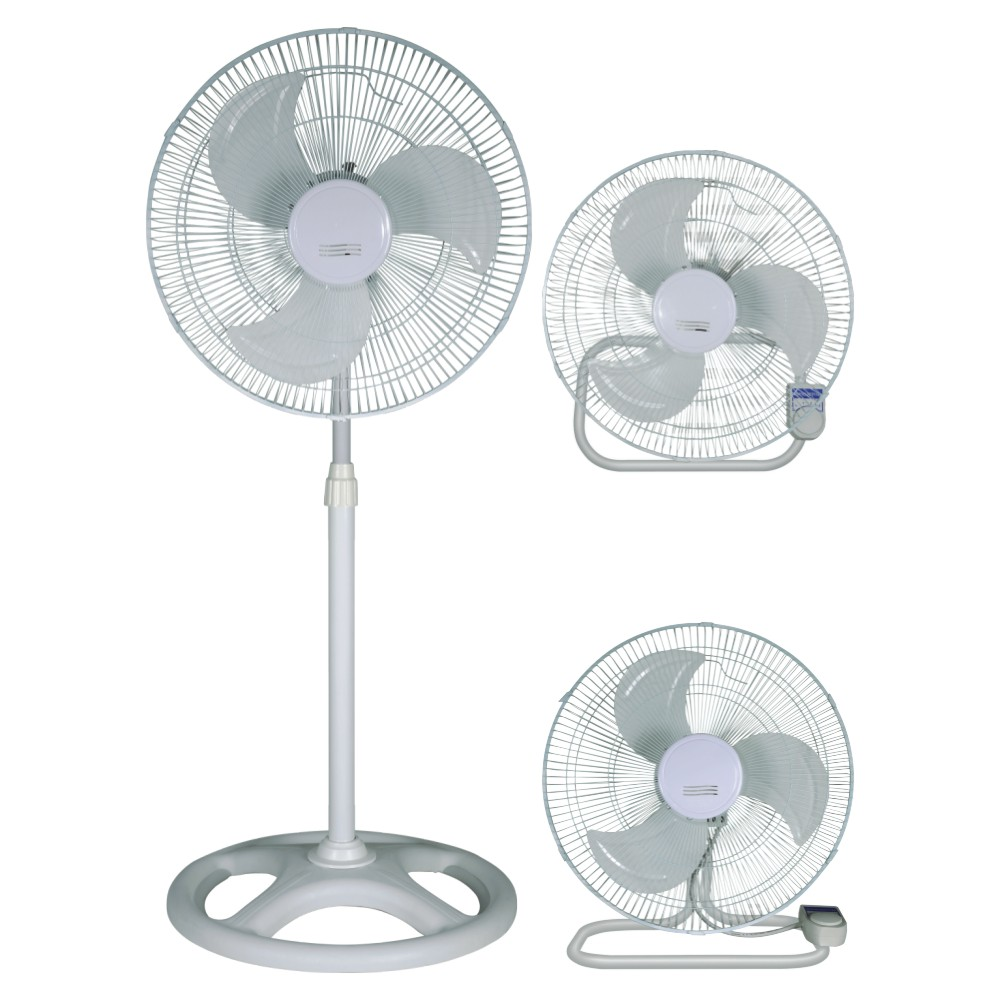
\includegraphics[width=0.5\linewidth]{fan.jpg}
  \caption{Electric fans}
  \label{fig:Electric fans}
\end{figure}

But rather than using fans for conventional use it can be used to help farmers in Sri Lanka. After getting the crops cut from the paddy fields rice seeds are mixed with airy seeds and other debris. Therefore they use the winnowing method of separation to remove airy seeds and debris from their crops.

\vspace{0.5 cm}

\begin{figure}[h!]
  \centering
  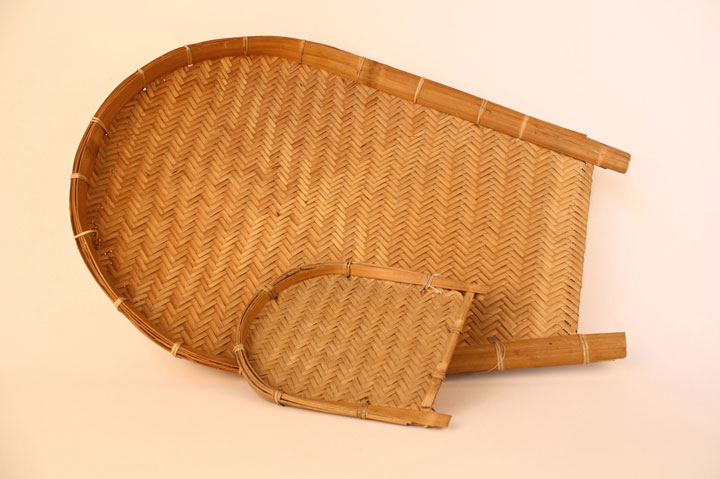
\includegraphics[width=0.5\linewidth]{winnowing fan.jpg}
  \caption{Winnowing fan}
  \label{fig:Winnowing fan}
\end{figure}

\begin{figure}[h!]
  \centering
  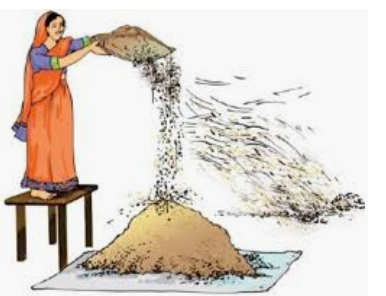
\includegraphics[width=0.5\linewidth]{winnowing seedss.png}
  \caption{Winnowing method of separation}
  \label{fig:Winnowing method of seperation}
\end{figure}

Winnowing is an agricultural for separate grain from chaff. It is also used to remove pests and weevils. Farmers let the mixture fall from a height and due to air flow in the field, different components in the mixture falls in separate places because of their variations of density. Good seeds falls near, while the debris and the airy seeds falls somewhere further. 

This is the normal procedure of farmers. But there are some challenges when using this method faced by farmers. Wind in the fields are not constant. Efficiency of removing debris and airy seeds gets reduce to this fact. Other reason is that this method can not be used in indoors due to low wind. 

We can overcome these problems by using a electric fan to create a artificial wind. This artificial wind is constant in speed and direction. Thus it would be highly efficient. And also it can be operated indoors. 

This method is an unconventional use of the electric fan. But using designing a new device suitable for rough use for this scenario will be a goof option for farmers. 

\newpage
\begin{figure}[h!]
  \centering
  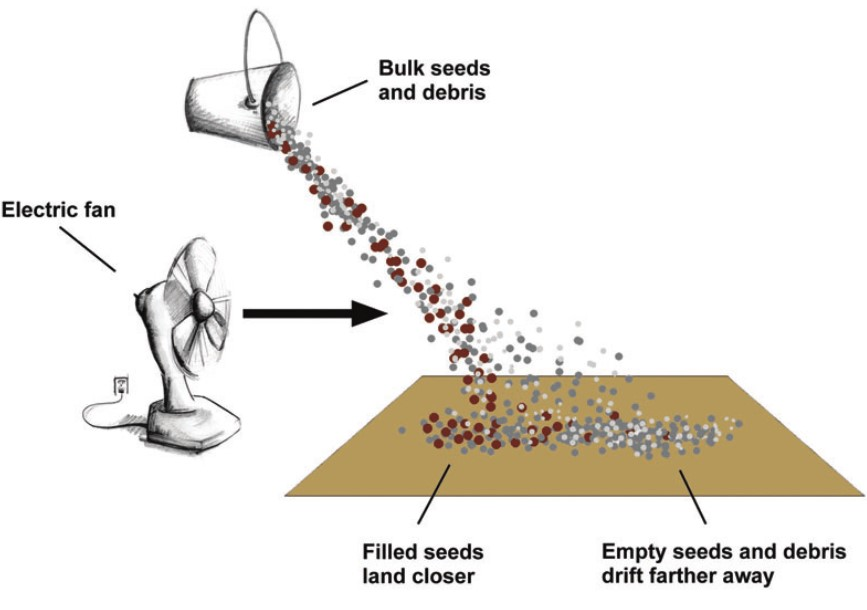
\includegraphics[width=\linewidth]{solution.jpg}
  \caption{Winnowing using electric fan}
  \label{fig:Winnowing using electric fan}
\end{figure}
\newpage


\section{People who would be addressed - Interpreters}

\begin{itemize}
    \item \textbf{Electric fan industry persons} - To get an understanding on feasibility
    \item \textbf{Technicians} - To know how to design a fan for rough use. 
    \item \textbf{Farmers} - To get to know there exact need. \textit{Ex:Height of the stand}
    \item \textbf{Agricultural Officers} - To know the rules and regulations of the agricultural equipments
    \item \textbf{Suppliers} - To get the materials for the device
    \item \textbf{Distributors} - Distribute all around the country
    \item \textbf{Market Professionals} - To get to know marketing strategies
    
\end{itemize}

\vspace{3 cm}
\begin{figure}[h!]
  \centering
  
\includegraphics[width=\linewidth]{interaction.png}
  \caption{Interpreters}
  \label{fig:Interpreters}
\end{figure}
\pagebreak

\section{How to convince customers to buy the product}
\begin{itemize}
    \item \textbf{Show them how easy to use it. Simple as an ordinary electric fan}
    \item \textbf{Show them how it increases the efficiency.}
    \item \textbf{Highlight the fact that it creates the constant wind without changing directions or speed}
    \item \textbf{Highlight how it can be used indoors}
    \item \textbf{Highlight the disadvantages in winnowing outside}
    \item \textbf{Even a small amount of rice seeds can be done using this at home}
    
\end{itemize}

\vspace{2 cm}
\begin{figure}[h!]
  \centering
  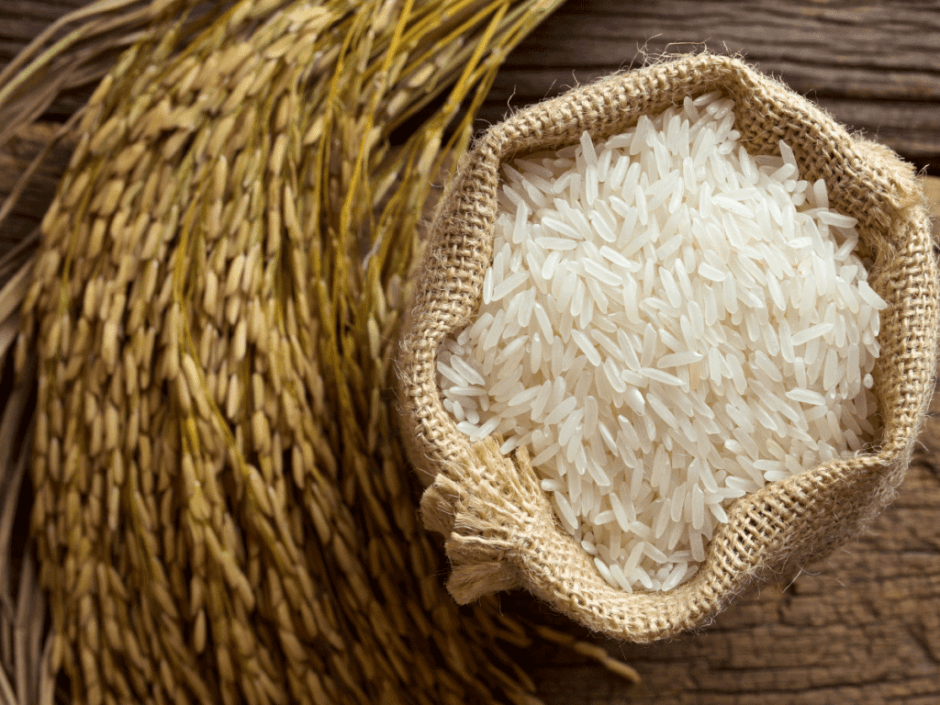
\includegraphics[width=\linewidth]{rice.png}
  \caption{Rice}
  \label{fig:Rice}
\end{figure}



\end{document}